%!TEX program = lualatex
%!TEX options = --shell-escape

\documentclass{beamer}

\usetheme{labss}

\usepackage{tikz}
\usetikzlibrary{positioning, decorations.pathreplacing, fit, calligraphy, arrows.meta, backgrounds, shapes.callouts, shadows.blur}
\usepackage[export]{adjustbox}

\usepackage{polyglossia}
\setmainlanguage{english}

\usepackage[style=authoryear, backend=biber, natbib=true]{biblatex}
\bibliography{rl_seminar}

\usepackage[french=guillemets*]{csquotes} %
\MakeOuterQuote{"}
\MakeAutoQuote{«}{»}

\usepackage{booktabs}
\usepackage{minted}
\usepackage{changepage}
\usepackage{relsize}

\title{
  \texorpdfstring{
    {\textcolor{black!25}{\hrule}}\vspace{4pt}
    Collaborating~like~professionals: integrating~NetLogo~and~GitHub
    \vspace{6pt}{\textcolor{black!25}{\hrule}}
  }{
    Collaborating~like~professionals: integrating~NetLogo~and~GitHub
  }
}
\date{August 23\textsuperscript{rd} 2018}
\author{Nicolas Payette}
\institute{Laboratory of Agent-Based Social Simulation, ISTC, CNR}

\titlegraphic{
\includegraphics[height=2em]{logo_labss}\quad
\includegraphics[height=2em]{logo_istc}\quad
\includegraphics[height=2em]{logo_cnr}\\[3mm]
\includegraphics[height=2em]{EC_H_pos.png}}

\newcommand\lbl[1]{\text{\footnotesize\begin{tabular}{@{}c@{}}#1\end{tabular}}}
\newcommand\st[1]{\hl{\larger #1}\par}
\newcommand\nt[1]{\textcolor{labss_bg}{#1}}

\begin{document}

\maketitle

\begin{frame}{Why version control?}\large
  \begin{center}
    \renewcommand{\arraystretch}{1.1}
    \begin{tabular}{l}
      \path{myModel.nlogo}\\\pause
      \path{myModel-v2.nlogo}\\\pause
      \path{myModel-v2.1.nlogo}\\
      \path{myModel-v2.2.nlogo}\\
      \path{myModel-v2.3.nlogo}\\
      \path{myModel-v2.3_temp.nlogo}\\
      \path{myModel-v2.3_temp_Aug2018.nlogo}\\
      \path{myModel-v2.3_temp_Aug2018_(edits).nlogo}\\
    \end{tabular}

    \pause\vfill\huge\hl{There is no excuse for this.}
  \end{center}
\end{frame}

{\setbeamercolor{background canvas}{bg=black}
\begin{frame}[plain]
  \centering
\includegraphics[height=\paperheight]{phd101212s.png}
\end{frame}}

\begin{frame}{What is version control?}\LARGE
  "Version control is a system that records changes to a file or set of files over time so that you can recall specific versions later."\footnote{\scriptsize\textcolor{black!50}{\url{https://git-scm.com/book/en/v2/Getting-Started-About-Version-Control}}}

  \vfill\larger
  It tracks \hl{who} changed \hl{what}, \hl{when}.

  \vfill\smaller
  The most used version control system is \hl{\texttt{git}}.
\end{frame}


\tikzset{
  node distance=5mm,
  decoration = {calligraphic brace, amplitude = 10pt},
  every node/.style = {rounded corners = 6pt, align = center, text width = 5em},
  arrow/.style = {very thick, -{Stealth}, draw=labss_bg},
  commit/.style = {draw=labss_bg!75, fill=labss_fg!50},
}

\newcommand{\Commit}[4]{
  \node [commit, #1] (#2) {#3\\\textcolor{labss_bg!90!black}{\texttt{#4}}};
}

\begin{frame}[fragile]{How \texttt{git} works: an overly simplistic illustration}
  \begin{description}
    \item[Repository:] A bunch of files and folders tracked by \texttt{git}.
    \item[Commit:] A snapshot of a repo with an author, a timestamp and a commit message.
  \end{description}
  \begin{center}
    \begin{adjustbox}{max width=\linewidth}
      \begin{tikzpicture}
        \Commit{}{c1}{Nicolas}{ce639ea}
        \uncover<2->{
          \Commit{right=of c1}{c2}{Nicolas}{ddc06df}
          \draw [arrow] (c1) -- (c2);
        }
        \uncover<3->{
          \Commit{right=of c2}{c3}{Nicolas}{c1509b2}
          \Commit{below=of c3}{c4}{Alice}{702c17f}
          \draw [arrow] (c2) -- (c3);
          \draw [arrow] (c2.south) -- (c4.west);
        }
        \uncover<4->{
          \Commit{right=of c3}{c5}{Nicolas}{02ee0b8}
          \Commit{right=of c4}{c6}{Alice}{92ecf3e}
          \draw [arrow] (c3) -- (c5);
          \draw [arrow] (c4) -- (c6);
        }
        \uncover<5->{
          \Commit{right=of c5}{c7}{Nicolas}{1ffc7de}
          \draw [arrow] (c5) -- (c7);
          \draw [arrow] (c6.east) -- (c7.south);
        }
        \uncover<6->{
          \Commit{right=of c7}{c8}{Nicolas}{972c491}
          \draw [arrow] (c7) -- (c8);
        }
      \end{tikzpicture}
    \end{adjustbox}
  \end{center}
  \uncover<7->{
    \par\bigskip
    \begin{description}
      \item[\texttt{git}:] A version control system.
      \item[GitHub:] A website that hosts \texttt{git} repositories.
    \end{description}
  }
\end{frame}

\begin{frame}{Why GitHub?}\large
  \st{It's big:}
  \begin{itemize}
    \item 29,904,101 users\nt{$^\star$}
    \item 21,490,796 public repositories\nt{$^\star$}\hfill\nt{$^\star$ as of August 15\textsuperscript{th} 2018}
  \end{itemize}
  \vfill\st{It's where the stuff we care about is being developed:}
  \begin{itemize}
    \item \url{https://github.com/NetLogo}
    \item \url{https://github.com/eclab/mason}
    \item \url{https://github.com/Repast}
    \item \url{https://github.com/JuliaLang}
    \item \url{https://github.com/python}
    \item Etc.
  \end{itemize}
\end{frame}

\begin{frame}[plain]
  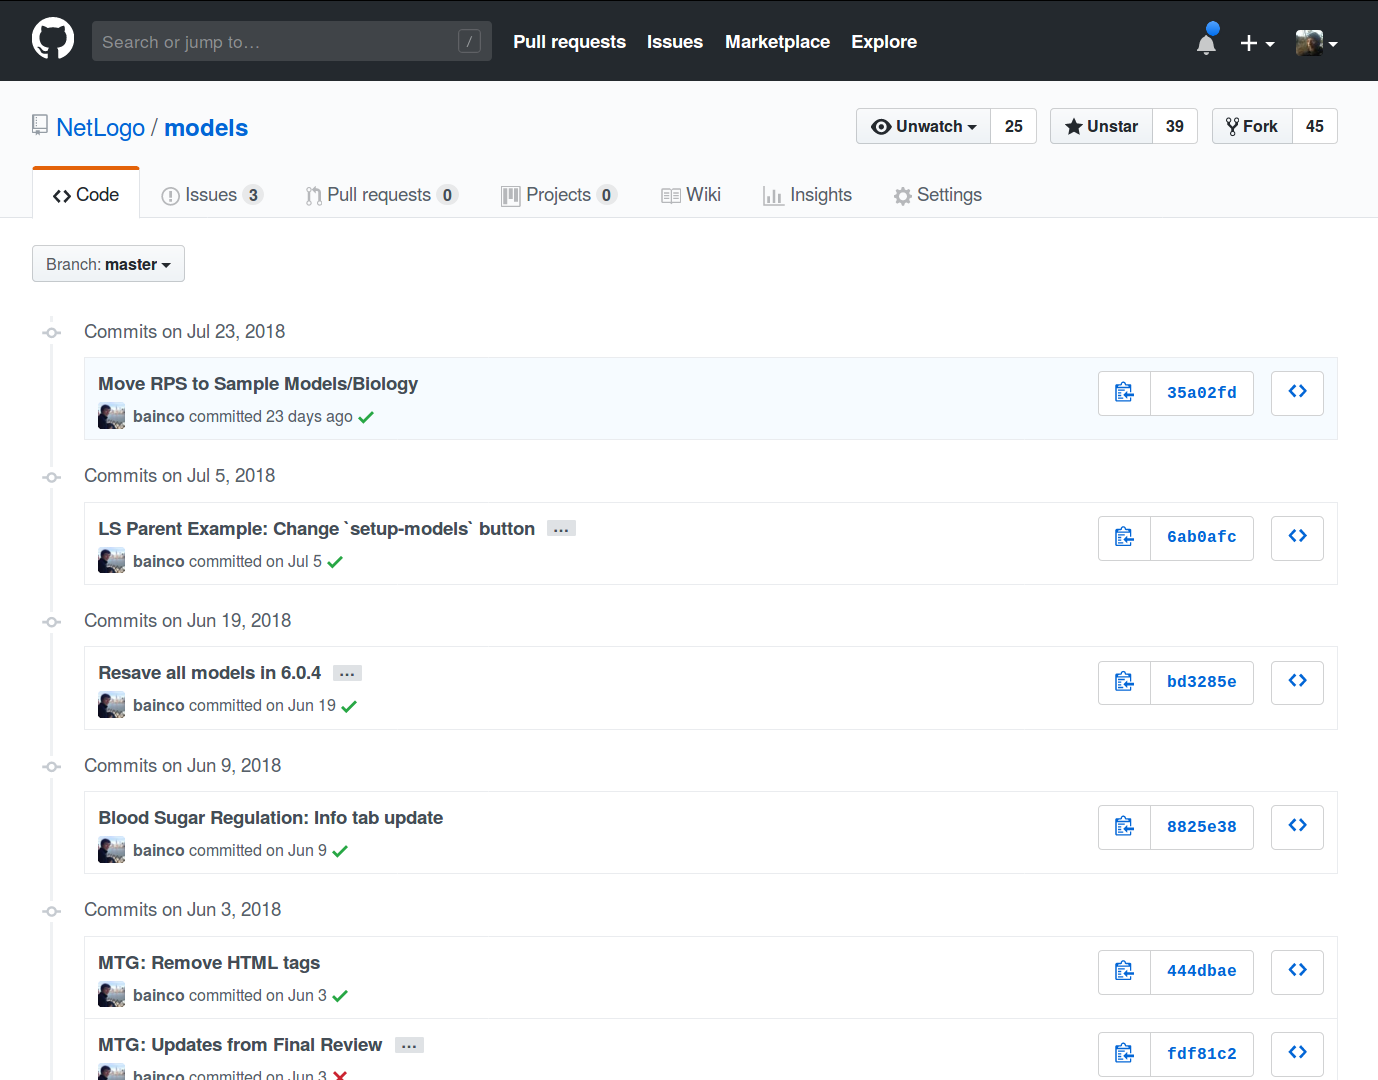
\includegraphics[width=\textwidth]{commits}
\end{frame}

\begin{frame}[plain]
  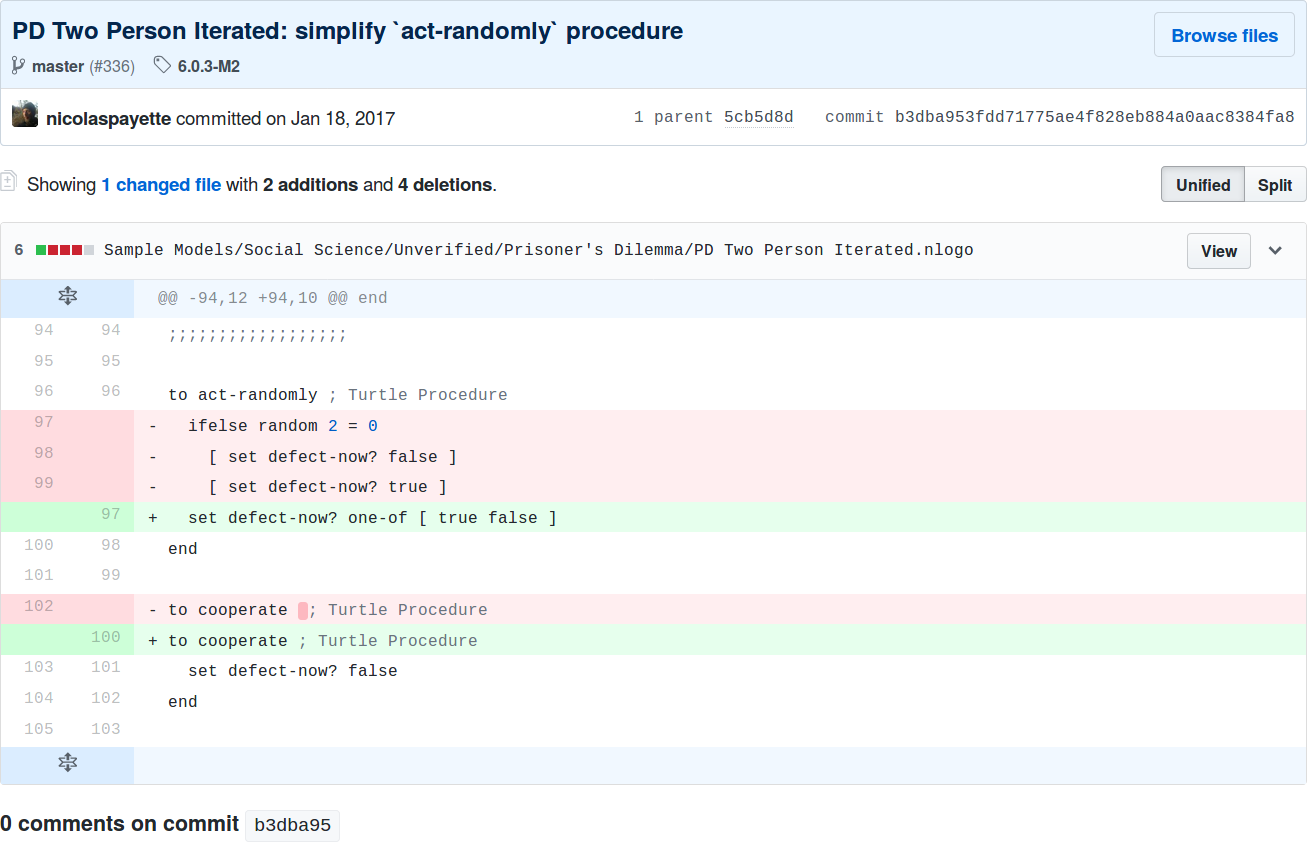
\includegraphics[width=\textwidth]{diffs}
\end{frame}

\begin{frame}{Why \emph{not} version control?}
  \centering
  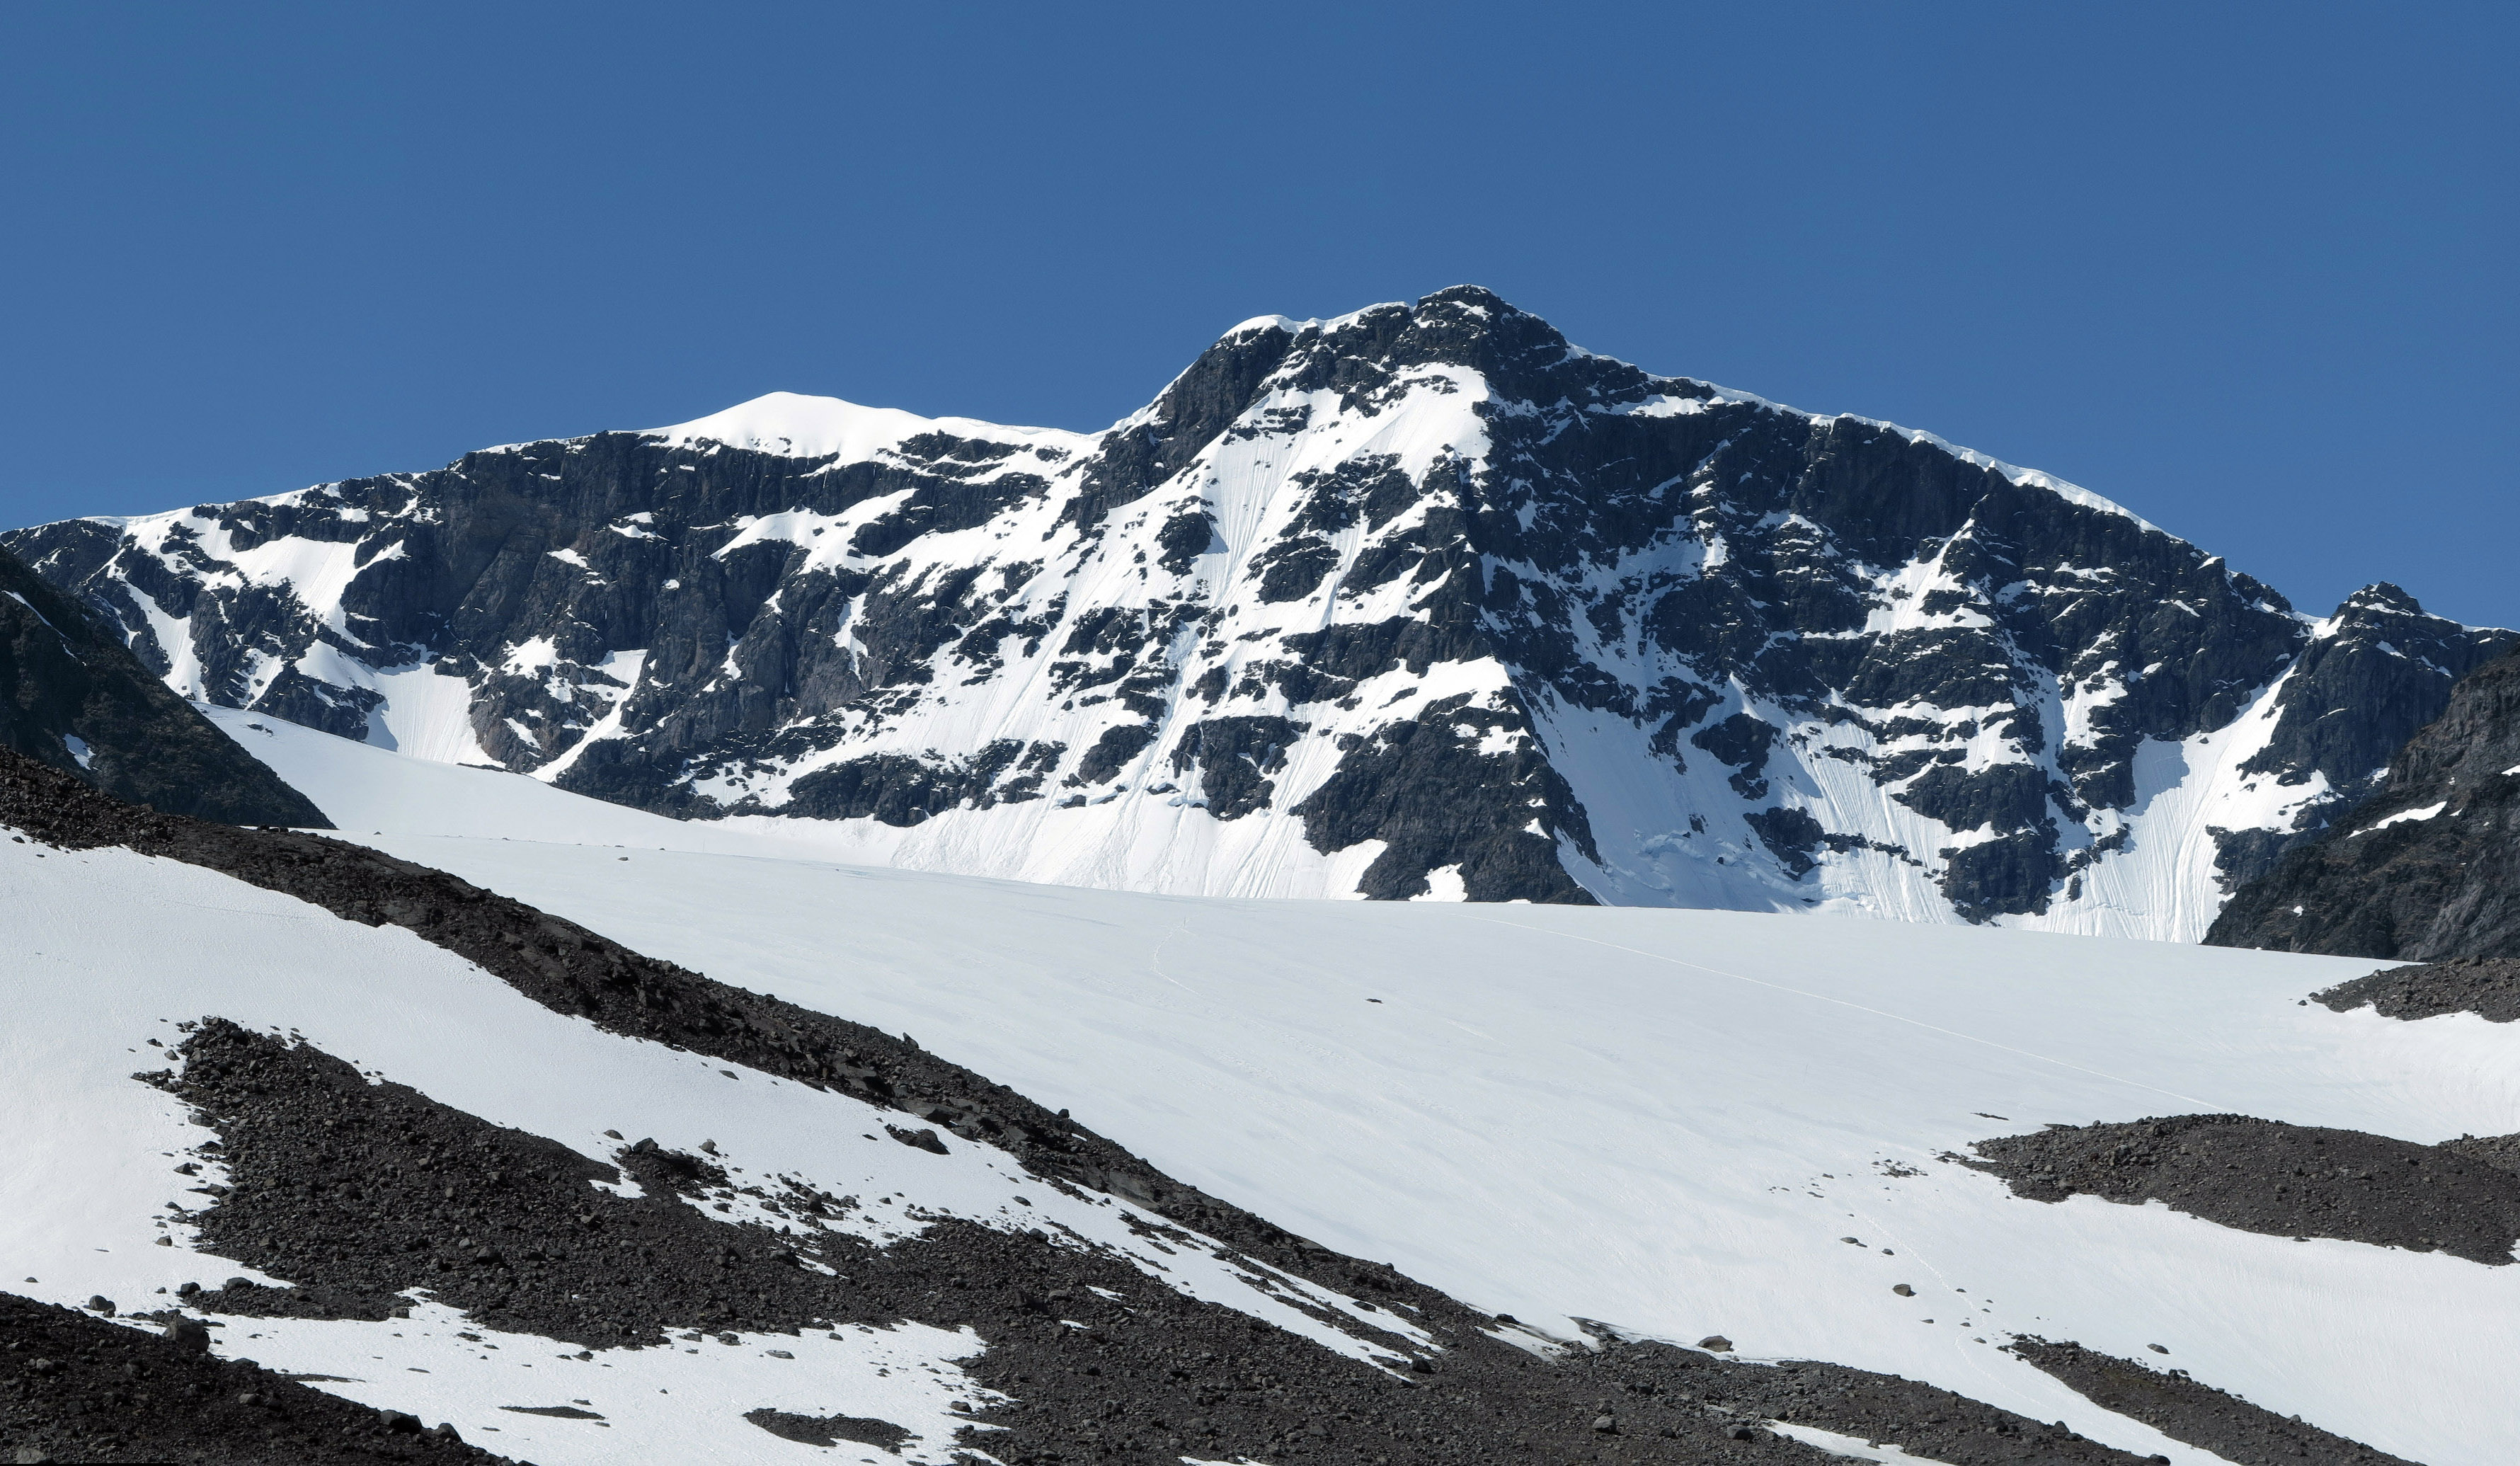
\includegraphics[width=\textwidth]{Kebnekaise.jpg}

  Kebnekaise, the highest peak in Sweden (2,106~m).\\
  \nt{\footnotesize (Photo by Alexandar Vujadinovic)}
\end{frame}

\begin{frame}
  \centering
  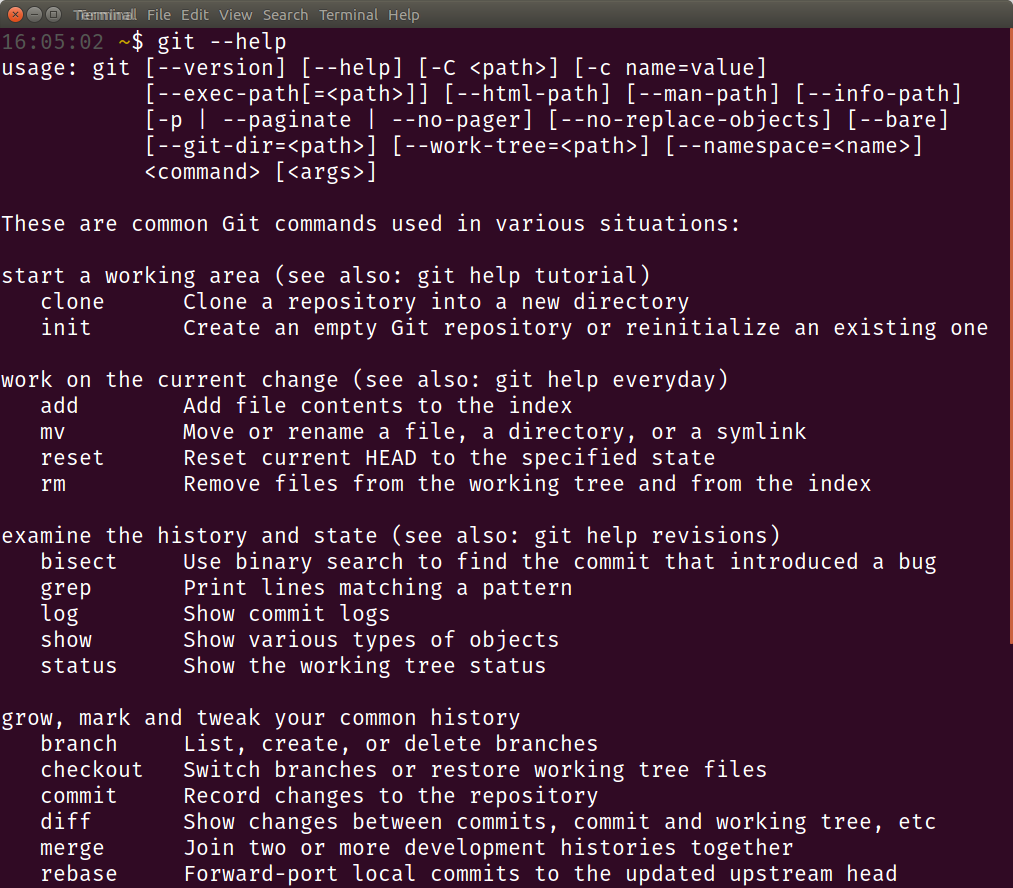
\includegraphics[height=\textheight]{githelp}
\end{frame}

\begin{frame}{Why not something else?}
  \begin{columns}\scriptsize
    \begin{column}[t]{0.5\textwidth}
      \begin{center}
        
\includegraphics[width=\linewidth]{openabm}

        \url{https://www.comses.net/}
      \end{center}
    \end{column}
    \begin{column}[t]{0.5\textwidth}
      \begin{center}
        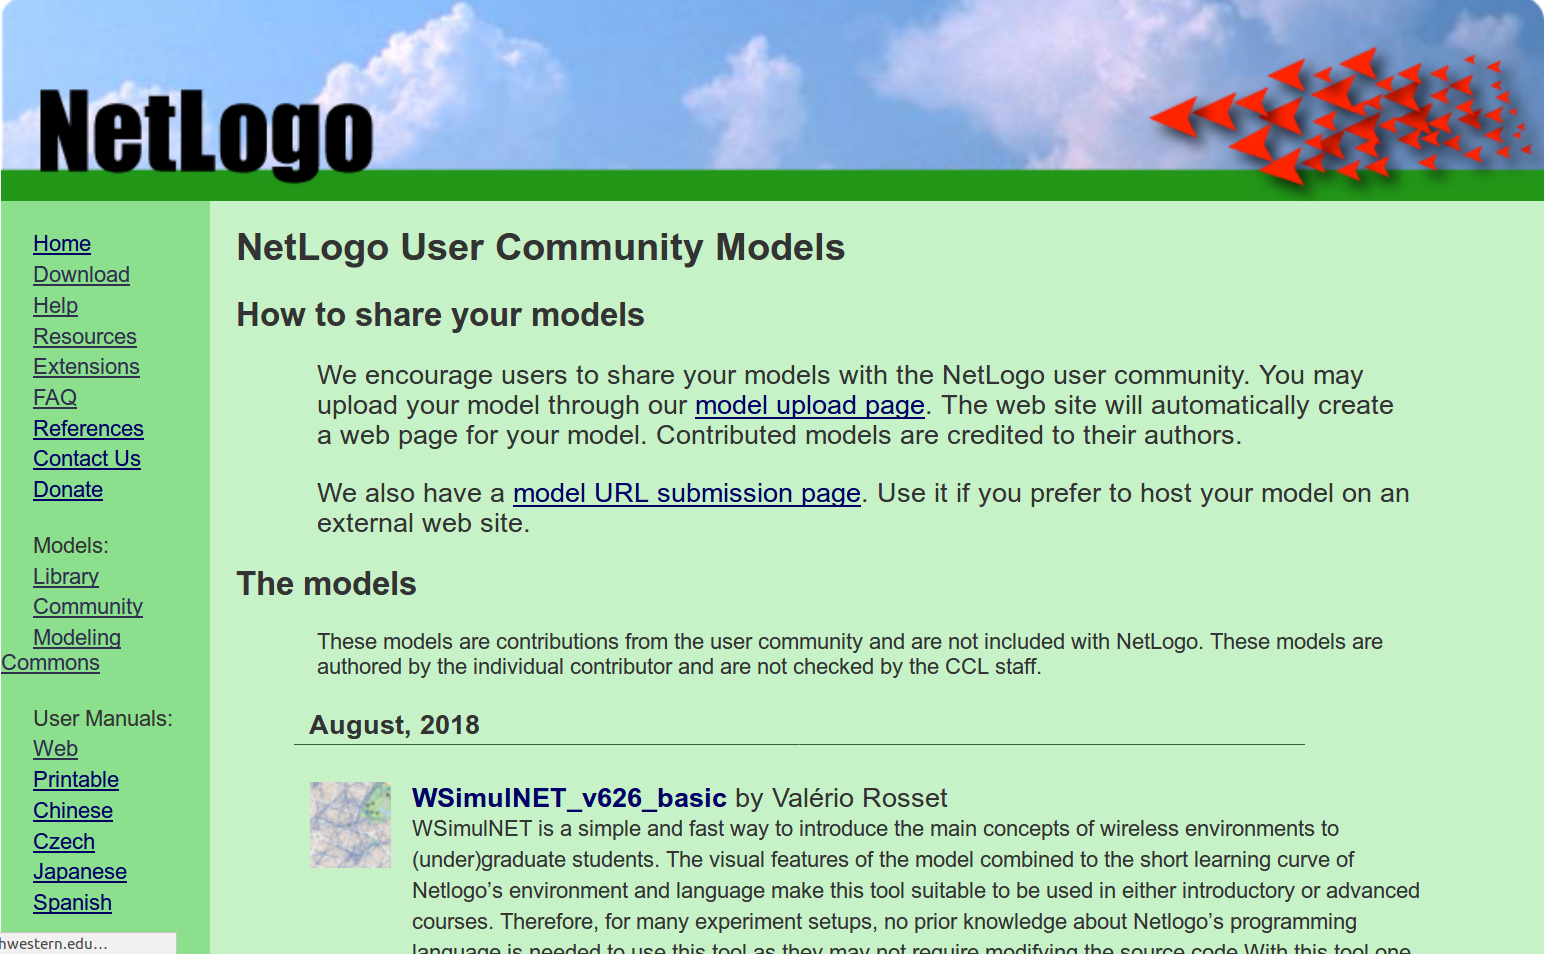
\includegraphics[width=\linewidth]{communitymodels}

        \url{http://ccl.northwestern.edu/netlogo/models/community/index.cgi}
      \end{center}
    \end{column}
  \end{columns}

  \pause\centering\huge\vskip1em
  Sharing, but no VC/collaboration.

\end{frame}

\begin{frame}{Why not the Modeling Commons?}
  \centering
  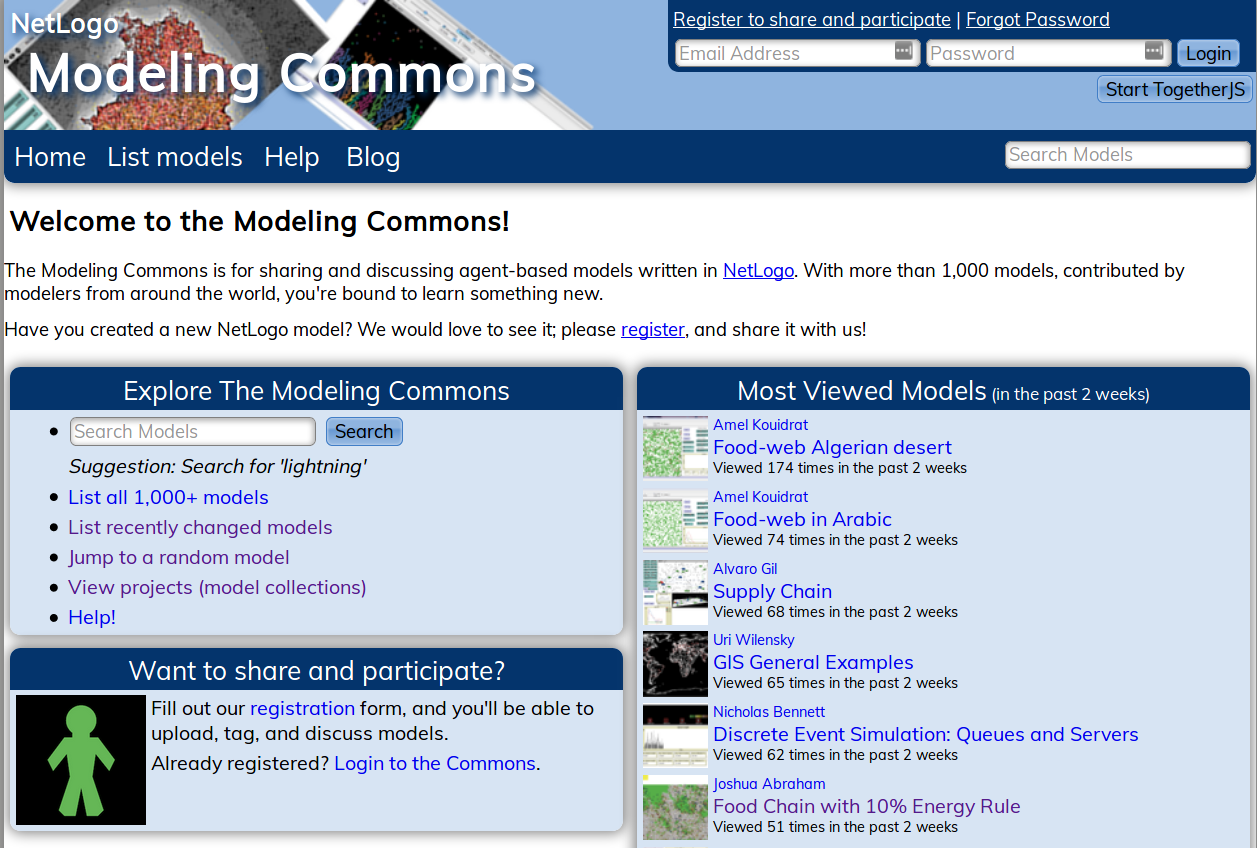
\includegraphics[height=0.6\textheight]{commons}

  \url{http://modelingcommons.org}
  \vfill\larger\pause

  NetLogo specific. Acquired skills are not transferable.
\end{frame}

\begin{frame}{What I want to do}

  \begin{columns}
    \begin{column}{0.5\textwidth}\Large
      \st{Short term:}
      \begin{itemize}
        \item Encourage modellers to upload their models to GitHub by making them easily discoverable from within NetLogo.
      \end{itemize}
      \st{Longer term:}
      \begin{itemize}
        \item Integrate some \texttt{git} features inside NetLogo.
      \end{itemize}
    \end{column}
    \begin{column}{0.5\textwidth}
      \begin{center}
        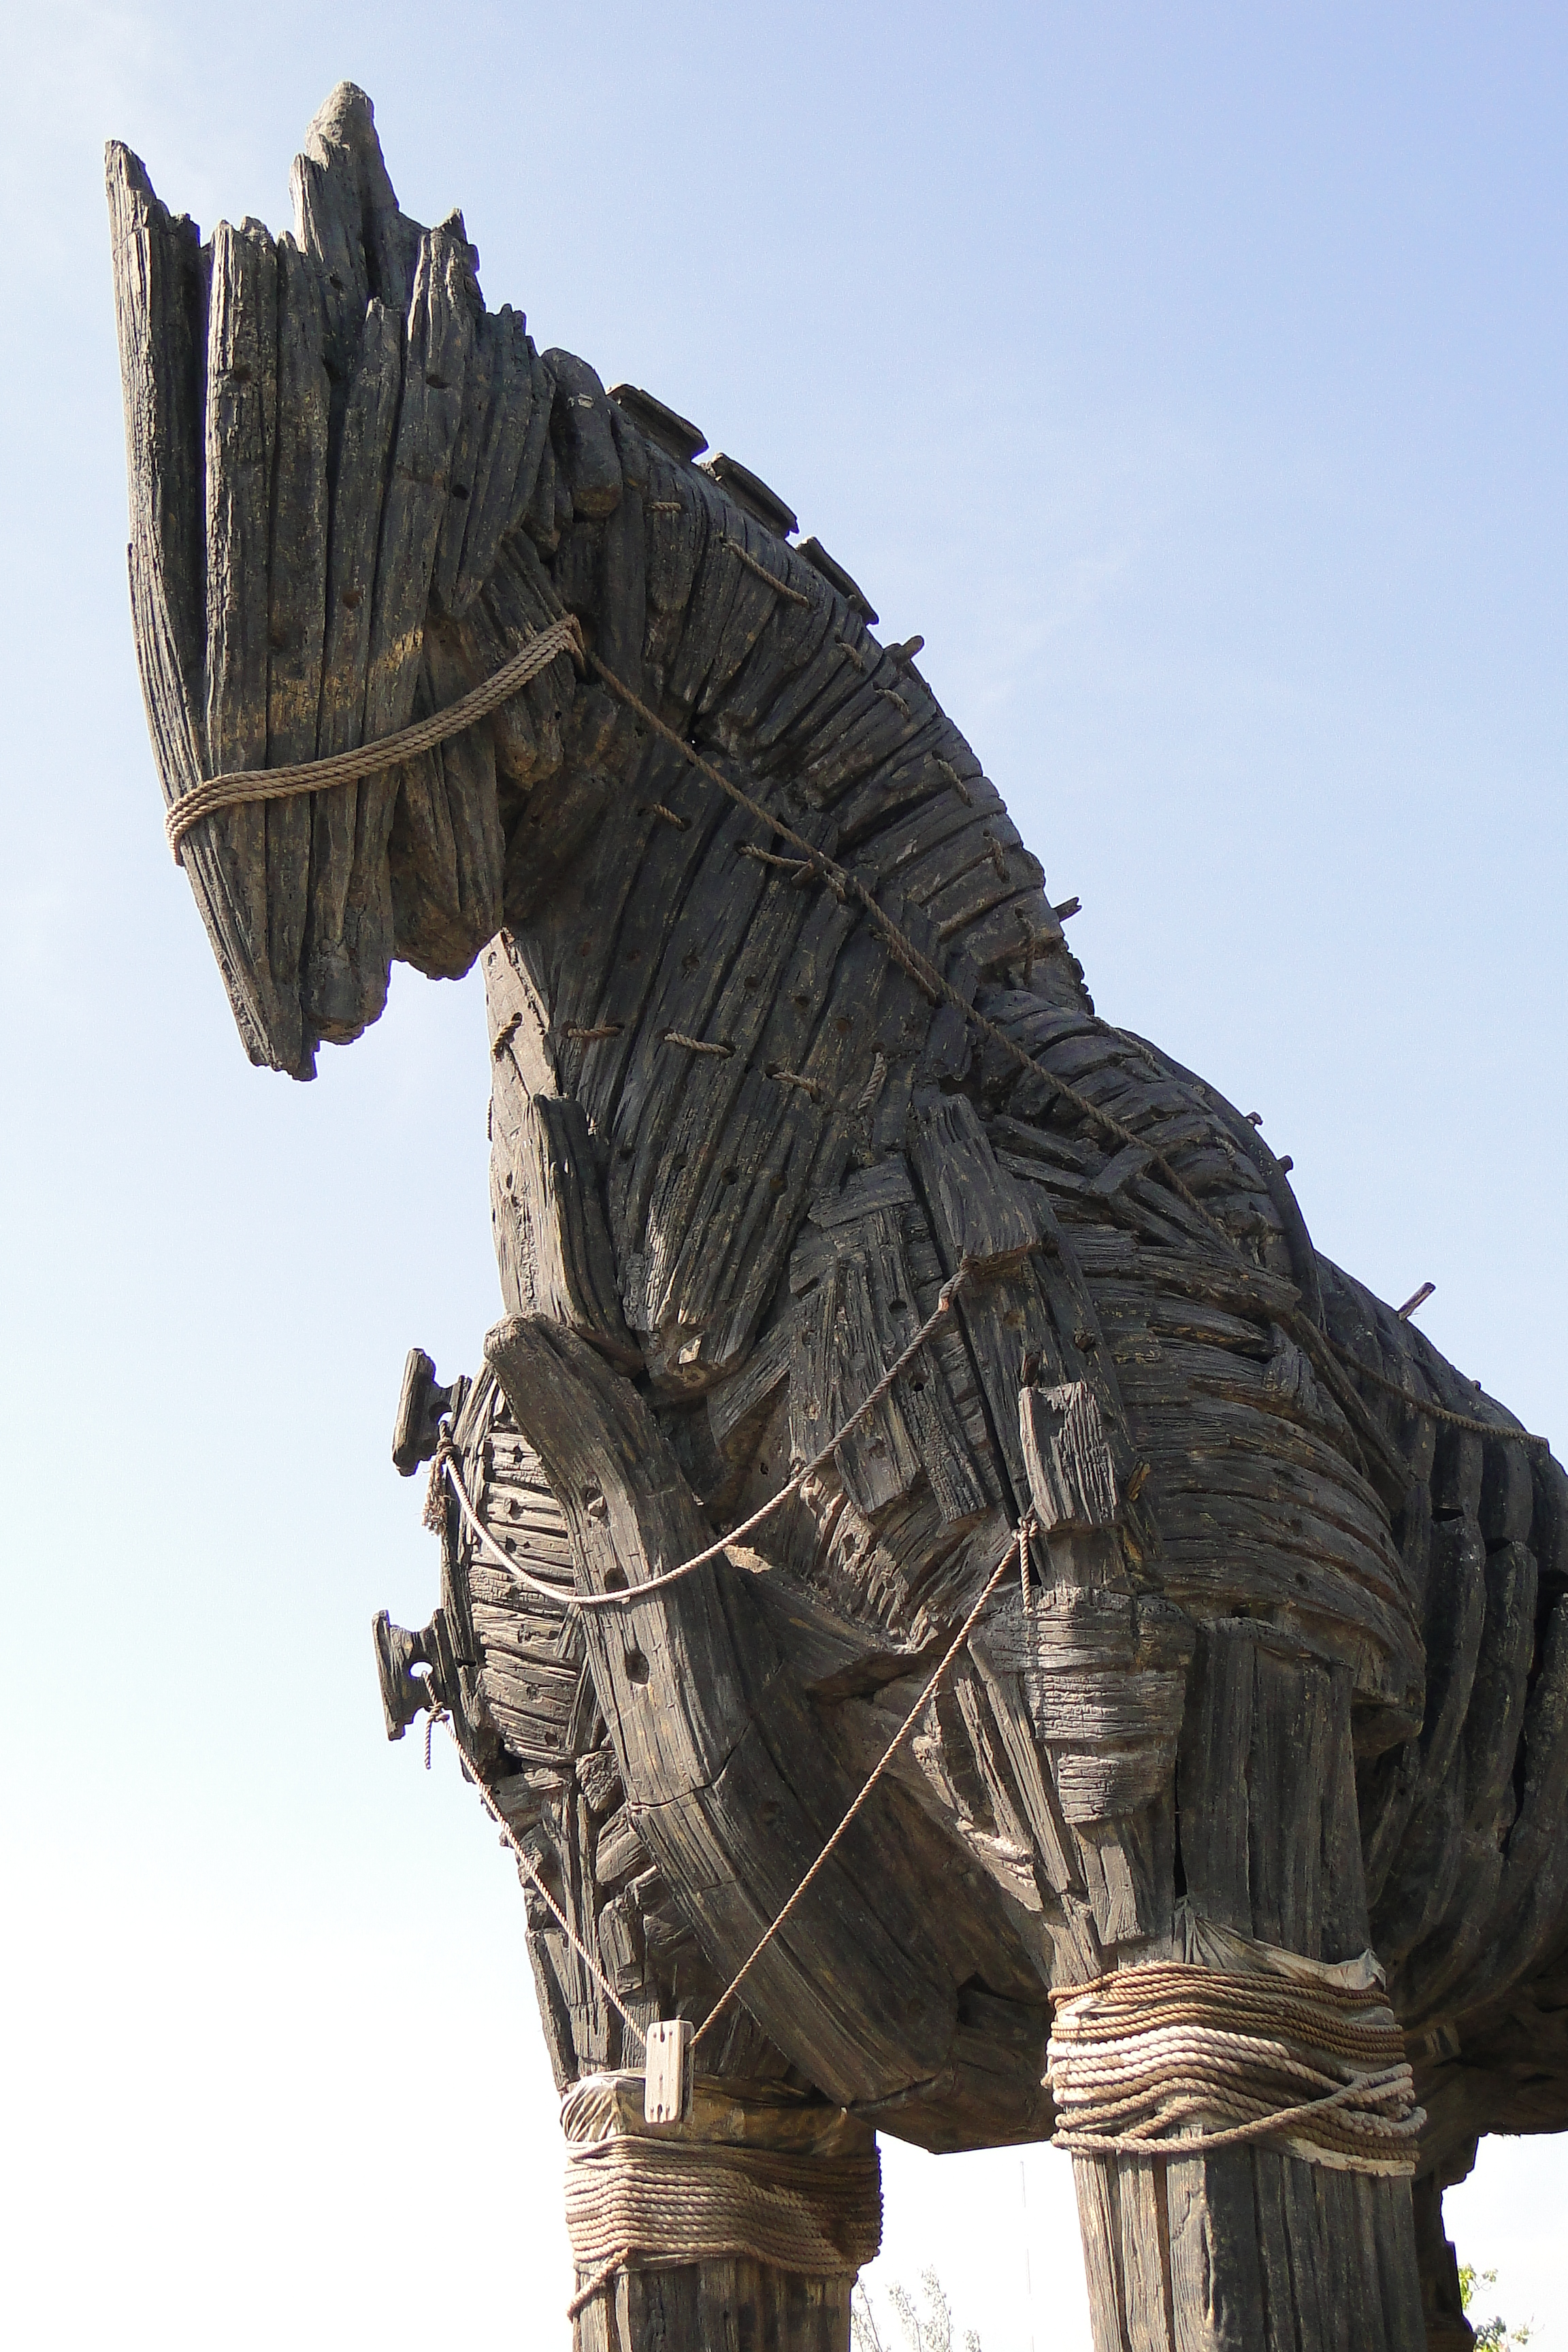
\includegraphics[height=0.7\textheight]{trojan}

        {\tiny \textcolor{black!50}{By Adam Jones from Kelowna, BC, Canada - Replica of Trojan Horse - Canakkale Waterfront - Dardanelles - Turkey, CC BY-SA 2.0, \url{https://commons.wikimedia.org/w/index.php?curid=64144380}}\par}
      \end{center}
    \end{column}
  \end{columns}

\end{frame}

\begin{frame}{The ``Online Models'' dialog}
  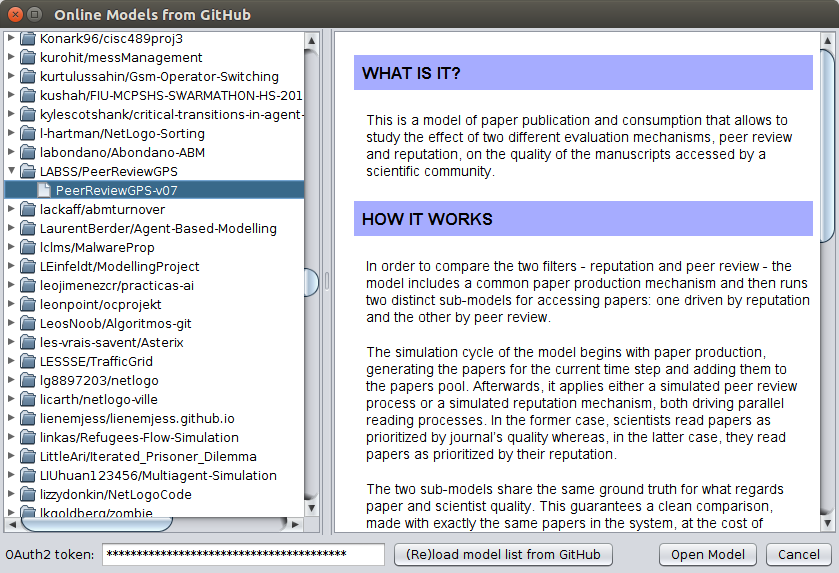
\includegraphics[width=\textwidth]{Screenshot}
\end{frame}

\begin{frame}{Future developments}\large
  \hl{\larger Technical stuff}

  \begin{itemize}
    \item Make it a plugin
    \item Improve UI, caching, authentification, etc.
  \end{itemize}
  \pause
  \vfill
  \hl{\larger Possible features}

  \begin{itemize}
    \item Upload current model to a new repo on GitHub;
    \item Commit changes and push them to GitHub;
    \item ``Fork'' someone else's model;
    \item Open ``pull requests'' for someone else's model;
    \item Show diffs between two versions of a model in the code tab.
  \end{itemize}
\end{frame}


\begin{frame}[fragile]\frametitle{How to try it}
  \begin{adjustwidth}{-6mm}{0mm}
    \hl{\larger From a bash terminal:}
    \vspace{1em}
    \begin{adjustwidth}{-12mm}{0mm}\footnotesize
      \begin{minted}{text}
        git clone -b online-models https://github.com/nicolaspayette/NetLogo.git
        cd NetLogo
        git submodule update --init
        ./sbt netlogo/run
      \end{minted}
    \end{adjustwidth}
    \vspace{2em}
    \hl{\larger For issues or suggestions:}

    \begin{itemize}\small
      \item \url{https://github.com/nicolaspayette/online-models/issues}
    \end{itemize}

  \end{adjustwidth}
\end{frame}

\end{document}
